
Consider the evolution of the $2\pi$-periodic square wave $\mathrm{sq} : \TT \to \R$, 
\[
	\mathrm{sq} (x)
		:= 
		\begin{cases}
			0
				&\text{if $0 < x < \pi$}, \\
			1 
				&\text{if $\pi < x < 2\pi$},
		\end{cases}
\]
under the linear Airy equation, 
\begin{equation}\tag{A}\label{eq:Airy}
	\begin{split}
		\partial_t u + \partial_x^3 u
			&= 0, \\
		u_{|t = 0}
			&= u_0. 
	\end{split}
	\end{equation}
Using Fourier series, we can explicitly compute the solution to the equation, 
	\[
		e^{-t \partial_x^3} \mathrm{sq} (x) 
			= \frac12 + \frac2\pi \sum_{j = 0}^\infty \frac{\sin((2j + 1)x - (2j + 1)^3 t)}{2j + 1}. 
	\]
In \cite{Olver2010}, Olver observed that this solution demonstrates a \textit{dispersive quantisation} effect, in the sense that at times $t$ with $\tfrac{t}{2\pi}$ irrational, the solution takes on a continuous fractal profile, while at times $t$ with $\tfrac{t}{2\pi}$ rational, the solution retains the piecewise constant character of the initial data; see Figures \ref{fig:olver1} and \ref{fig:olver2} taken directly from \cite{Olver2010}. 

The dispersive quantisation is more broadly known in optics as the \textit{Talbot effect}, owing to the early experimental observations of Talbot \cite{Talbot1836}. For general linear dispersive equations posed on the torus, the Talbot effect predicts that the qualitative features of the solutions depend on the number-theoretic properties of time. These result follow from well-known results concerning exponential sums. We will focus on the following result of Oskolkov \cite{GoncharSaff1992}, 

\begin{figure}[h]\label{fig:olver1}
	\begin{center}
		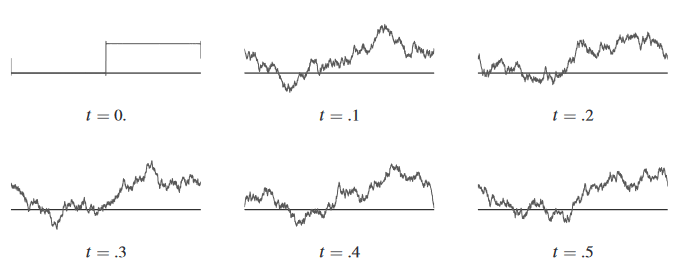
\includegraphics{graphics/olver1}
	\end{center}
	\caption{Approximate solution to \eqref{Airy} with square wave initial data $u_0 (x) = \mathrm{sq}(x)$ at irrational times. The Fourier series is computed to the first 1000 terms.}
\end{figure}


\begin{figure}[h]
	\begin{center}
		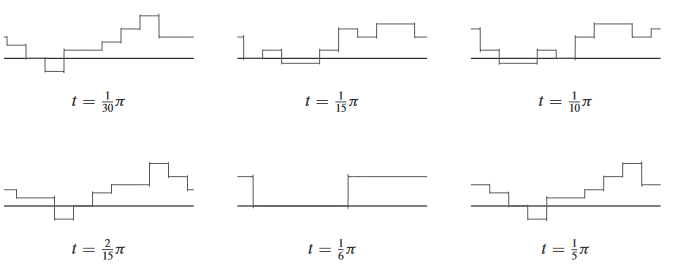
\includegraphics{graphics/olver2}
	\end{center}
	\caption{Approximate solution to \eqref{Airy} with square wave initial data $u_0 (x) = \mathrm{sq}(x)$ at rational times. The Fourier series is computed to the first 1000 terms.}\label{fig:olver2}
\end{figure}

\begin{theorem}[Linear Talbot effect]\label{thm:talbot}
	Let $u_0 \in \mathrm{BV} (\R/2\pi \Z)$ be a $2\pi$-periodic function of bounded variation. Then the solution 
		\[
			u(t, x) 
				:= \sum_{k \in \Z} \widehat u_0 (\xi) e^{i k^3 t} e^{i k x}
		\]
	to the linear KdV equation with initial data $u_0$ has the following properties: 
	\begin{enumerate}
		\item The uniform bound
			\[
				||u||_{L^{\infty}_{t, x}} 
					\lesssim ||u_0||_{L^\infty_x} + ||u_0||_{\mathrm{BV}}, 
			\]
		
			\item For each $t$ such that $\tfrac{t}{2\pi} = \tfrac{p}{q}$ for $p, q \in \Z$ coprime, $u$ has $Nq$-many discontinuities in $x$, where $N \in \overline \N$ is the number of discontinuities of $u_0$. \label{item:rational}
        
			\item For each $t$ such that $\tfrac{t}{2\pi}$ is irrational, $u$ is a continuous function of $x$.
	\end{enumerate}
	In particular, if $u_0$ is continuous, then $u \in C^0_{t, x} (\R \times \TT)$. 
\end{theorem}

\begin{proof}[Proof of \ref{item:rational}]
	One can write the solution as a linear combination of translated initial data with coefficients given by Gauss sums, 
	\[
			e^{-t \partial_x^3} u_0 
				= \frac1q \sum_{j = 0}^{q - 1} \mathsf G_{p, q} (j) u_0 \left( x - 2\pi \tfrac{j}{q} \right),
		\]
	where 
		\[
			\mathsf G_{p, q} (j)
				:= \sum_{\ell = 0}^{q - 1} e^{-2\pi i \ell^3 \frac{p}{q}} e^{2\pi i \ell \frac{j}{q}}.
		\]
\end{proof}

While we will not explore it further, to give another example let us cite the Besov smoothing result of Kapitanski-Rodnianski \cite{KapitanskiRodnianski1999}, 

\begin{theorem}[$B^{s, \infty}_\infty$-regularity of the Schr\"odinger fundamental solution]
	Denote the fundamental solution of the Schr\"odinger equation on the torus by 
		\[
			E_t (x) 
				:= \sum_{k \in \Z} e^{i k^2 t} e^{ikx}. 
		\]
	Then 
		\begin{enumerate}
			\item For $t$ such that $\tfrac{t}{2\pi}$ is rational, $E_t \in B^{-1, \infty}_\infty (\TT)$. 
			\item For $t$ such that $\tfrac{t}{2\pi}$ is irrational, $E_t \in B^{-\frac12-, \infty}_\infty (\TT)$. 
		\end{enumerate}
\end{theorem}

For a survey on manifestations of the linear Talbot effect, see 
\cite[Chapter 2.3]{ErdoganTzirakis2016} and \cite{Olver2010}. 

In this note, we will be concerned with justifying the Talbot effect for non-linear perturbations of dispersive equations, namely the KdV equation, 
\begin{equation}\label{eq:KdV}\tag{KdV}
	\begin{split}
		\partial_t u + \partial_x^3 u + 6 u \partial_x u 
			&= 0,\\
		u_{|t = 0}
			&= u_0. 
	\end{split}
	\end{equation}
This equation is invariant under the Galilean transformation 
		\[
			u(t, x) \mapsto (t, x - vt) + \frac{v}{6},
		\]
and, due to the total derivative non-linearity, conserves momentum, 
	\[
		M[u]
			:= \int_{0}^{2\pi} u(t, x) \, dx
	\]
Thus, one can assume without generality that our solution has mean zero $\widehat u(0) \equiv 0$ for all time. This normalisation will be convenient for our analysis. We will present two perspectives on the matter of non-linear dispersive quantisation.

The first draws from \cite{ErdoganTzirakis2013}, in which Erdogan-Tzirakis observed a smoothing effect for the difference between the non-linear and linear flows. In particular, this difference is spatially continuous for bounded variation data, allowing one to conclude Theorem \ref{thm:talbot} persists for \eqref{KdV}. This is the subject of Section \ref{sec:smooth}. 

The second point of view is phenomenological; namely the question of whether we can see the non-linear Talbot effect from numerics. General numerical methods require a high degree of regularity to guarantee smoothness, however, in this setting it is of interest to study data below the threshold of energy arguments $H^{3/2} (\TT)$. It was recently shown by Rousset-Schratz \cite{RoussetSchratz2022} that, using discretised Fourier restriction norm estimates, one can construct numerical schemes which do in fact converge for rough data $u_0 \in H^{0+}( \TT)$. This is the subject of Section \ref{sec:numerics}. 